

This chapter is dedicated to the fundamental concepts and current research in different areas related to this project: radiation environment, radiation effects on SRAM-FPGAs, single-event upsets, fault-injection, signatures,  and behavioral fault modeling. All of these topics are relevant for the purpose of this research --- ideally, places itself as an attractive research project.





%The potential analysis of a malfunction due to radiation encourages manufacturers to invest more and more in the development of the design tools that allows the choice of the mitigation strategies. In the 1980s,
%components have begun to be developed for space applications and Aviation
%In the 1990s, the explosion of the development of consumer electronics multiplied
%Commercial Off-The-Shelf (COTS) components, which are
%economical and available in large quantity. Further,  the reduction
%of the transistor sizes, the intrinsically small transistor is less sensitive to
%radiation. But because of its smaller sensitive surface, the opposite effect is observed at the level of an integrated circuit. Indeed, the sensitivity of the components increases while the ability of
%engraving decreases despite the gain brought by the miniaturization. The two main factors
%of this conjecture are the increase in the density of integration and the
%threshold voltages of the transistors. For the last ten years or so, studies have been able to provide the evidence of the potential sensitivity of integrated circuits at high altitude commercial flights \cite{normand1998extensions}. This is particularly the case for complex components with high integration such as
%those based on Static Random Access Memory (SRAM) \cite{baumann2005radiation}, which is the target technology for this project. The aerospace industry is looking for the solutions that offer an acceptable compromise between radiation reliability and the system cost, including those based on user-programmable integrated circuits based on static memory. The search for such solutions has implications for the complete flow of design and development of embedded systems. Indeed, this requires the designers to check design robustness to the radiations design. For this purpose, simulation tools that allow the injection of faults in the design is being used. But simulation-based verification has its limits, long testing time is added to the conventional verification, which is already considered to the bottleneck of the design process. The system, once implemented, should also be subject to costly laboratory testing using particle accelerators. To provide a cost-effective fault emulation techniques were developed by our research group ~\cite{hobeika2014multi,  bocquillon2009evaluation,souari2015optimization}.



\section{Radiation Environment}


The electronic systems operate in the space are exposed to radiations. The first evident were observed in the sixties, but it was difficult to separate soft-error from the other form of interference. The first evidence of malfunctions in electronic circuits embarked in spacecraft caused by the radiations reported in May 1979 \citep{may1979alpha}. In the outer space, there are three main types of radiative sources that effect the Earth's atmosphere.

\begin{itemize}

\item Galactic cosmic rays.

\item Radiation from the sun, i.e., solar wind and solar flares.

\item Earth's magnetic field, e.g., magnetosphere and radiation belts.

\end{itemize}


\subsection{Galactic Cosmic Rays} 

The origin of cosmic rays is hardly known. However, we have information about they are energetic particle spread throughout the galaxy including the solar system \citep{SWE20216}. This radiation comes from sources present "in and out" of our
universe. Interactions of these radiations with an interstellar matter, shock waves, and electromagnetic fields, accelerate these radiations. As a result, at the scale of our
solar system, it appears as an isotropic angular distribution, and the particles are ionized~ \citep{SWE20216}. The sun is also the origin of some of these particles, but most of them come from the galactic sources known as galactic cosmic rays (GCR).
Cosmic radiation was discovered by V. Hess in 1912 through measurements made from balloon probes \citep{cronin1999cosmic}. The cosmic rays constitute of 85\% of the proton that is nuclei of the hydrogen atom, 12\% are alpha particles that are helium nuclei, and the others are electrons and nuclei of heavier atoms. The energy of cosmic rays ranges from 1GeV to 108 TeV. 


\subsection{Radiation from the Sun} 

The sun alone accounts for 99.8\% of the total mass of the solar system, the remaining 0.2\% other planets. The sun is mainly composed of hydrogen 90\% and helium 8\%~\citep{wikisun}. In the center of the sun, thermonuclear fusion reactions convert hydrogen into helium. The energy produced on this occasion is emitted in the form of radiation and particles. The radiation produced by the sun has two essential sources: solar flares and solar winds. 

\subsubsection{Solar Flares} 

The activity level of the sun is never constant but follows a cyclical variation that composed of active years followed by calm (no activity) years. The period of recent solar cycles has
varied between 9 and 13 years, with an average of about 11 years \citep{nasa}. The last maximum solar activity is observed in April 2014 period of the "solar-cycle" started in 2008 \citep{nasa}. The activity of solar cycles is frequently measured by the "number of sunspots observed." The first sunspot was observed in 1610 by Galileo while he devoted himself to the observation of the sun. The number of sunspots varies cyclically, and most sunspots events are
generating protons appear during active solar years. During a solar cycle of 11 years, there are 4 years of low activity, and 7 years of strong activity, punctuated by sporadic emissions of large particle fluxes, In this radiative context, there are two types of solar flares: \\
- Proton solar flares, lasting from few hours to few days, and primary emission consists of protons of significant energy (up to
a few hundred MeV). \\
- Solar flares: the main emission consists of heavy ions.

\subsubsection{The Solar Wind}

The solar wind begins in the solar corona, where temperatures are in millions of degrees, gives electrons enough energy to allow them to
escape from the gravitational field of the Sun. In reaction, protons and heavy ions are also ejected. The Sun evacuates about $10^{14}$ kilograms of material each day. 


\subsection{The Earth's Magnetic Field}

The Van Allen radiation belts are two toroidal zones of energetic particles that are held around the magnetic field of the Earth. The magnetosphere is the region surrounding a celestial object in which the
physical phenomena are dominated or organized by its magnetic field. These radiation belts are composed of energetic protons and electrons coming from solar wind and cosmic rays. There are two belts named --- inner belt and outer belt. The inner belt is composed of protons and electrons and outer belt is composed of energetic electrons~\citep{barth2003space}


\subsection{Influence of Radiations}
The previously mentioned sources of particulate matter influence only persons and equipment
outside the Earth's atmosphere. However, since 1992, the year of observation of the first
bit-flipped in-flight memory~\citep{taber1995investigation, taber1993single} observed. It has been demonstrated that the particles responsible for these
phenomena are atmospheric neutrons~\citep{leray2004atmospheric, jedec2006measurement}.
One more incident reported in~\cite{SWE20216} about the neutron influenced aircraft's operation of the flight from Singapore to Perth started incorrect values, after the investigation: SEE resulting from the high-energy atmospheric neutrons were interacting with the integrated circuits.
Atmospheric neutrons are the result of the collision of cosmic radiation,
mainly protons, with the atoms present in the upper atmosphere of the Earth. The result of these collisions is either the formation of ionized particles or a nuclear reaction which
produced mainly neutrons, protons, electrons, etc. These phenomena are called
"Atmospheric shower" as shown in Figure~\ref{shower}. The product resulting from these collisions is the generation of
protons, neutrons, muons, etc. Since neutrons are uncharged particles, they do not
cause  - operational failure directly of electronic devices. However, they can generate kernels of recoil in
the material they cross. When these ions originate in the active zones of the integrated circuit, they can modify the normal behavior of the components~\cite{normand1998extensions}.
%


\begin{figure}[h]
 \centering
  \captionsetup{justification=centering}    
   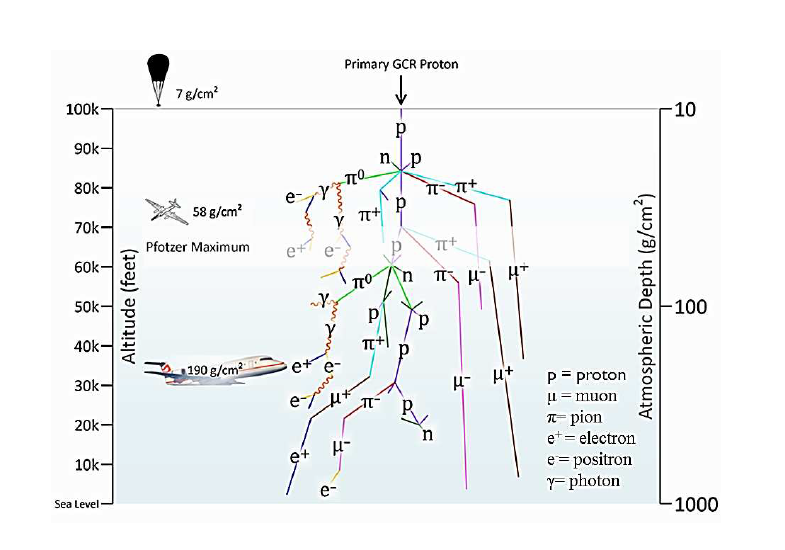
\includegraphics[scale=0.75]{Figures/showerplusaircraft.png}
  \caption{Cosmic rays shower~\cite{ziegler1996ibm}.}
\label{shower}
\end{figure}


\subsubsection{Neutron interactions}



The neutron is a particle without electric charge but with a mass. When a high-energy neutron moves through a silicon substrate, charged particles are produced. If the charge of these particles is sufficient enough, then they can alter the state of the static memory.  For avionics the \textbf{neutrons} are the dominant particles~\citep{xilinnseu}. Neutrons are measurable at the altitude of 330 KM and their density increases until it reaches around 40 Km altitude (Future's aircraft flying altitude). However, the density decreases below the 40 Km altitude and about 500 times lesser at ground level as compare to 40 Km altitude. Until 90's the neutrons with energy above 100 MeV were considered dangerous for electronics components. But due to the shrinking the transistor size, circuits are now become more sensitive to the low energies as well.   

\subsection{Fault Caused by Cosmic Rays in Digital Circuits}


Ionizing particles can interact with an embedded electronics and have critical consequences for the success of a space mission or avionics altitudes flights. The interaction causes two types of effects ---
single event effects (SEE) (caused by a single particle) and the total ionizing dose (long-term radiation effects, mostly due to electrons and protons). In this research work, we mainly focused on the SEEs.


A Single Event Effect (SEE) results from a single energetic particle. When the particle strikes a sensitive node in a semi-conductor device, the ionization by the particle might produce a current pulse inside the device, which might cause soft or hard errors in the configurtaion memory of the device. Results in data corruption, transient disturbance, high current conditions (non-destructive and destructive
effects). If SEE cannot handle well cause unwanted functional interrupts or in worst case catastrophic failures. Commonly, SEEs include: single event upset (SEU), single event latch-up (SEL), single event burn-out (SEB), and single event transient (SET) etc as mentioned in Table~\ref{SEE-Summary}. 


\begin{table}
\caption{Single Event Effects Summary~\cite{manuzzato2010single}}
\centering
\label{SEE-Summary}
\scalebox{0.7}{

   \begin{tabular}{c|c|c}
         \toprule
    \hline
     
     Single Event Upset (SEU)                  & corruption of the information \\ & stored in a memory element            & Memories, latches in logic devices                                  \\ \hline
    
    Multiple Bit Upset (MBU)                  & several memory elements \\ & corrupted by a single strike                & Memories, latches in logic devices                                  \\ \hline
    Single Event Functional Interrupt (SEFI) & corruption of a data path      & Complex devices with built-in state       \\ \hline
    Single Hard Error (SHE)                   & unalterable change of state in\\ & a memory element                     & Memories, latches in logic devices                                 \\ \hline
    Single Event Transient (SET)              & Impulse response of certain\\ & amplitude and duration                  & Analog and Mixed Signal circuits                      \\ \hline
    Single Event Disturb (SED)                & Momentary corruption of the\\&information stored in a bit             & combinational logic, latches in logic devices                       \\ \hline
    Single Event Latchup (SEL)                & high-current conditions                                              & CMOS, BiCMOS devices                                                \\ \hline
    Single Event Snapback (SESB)              & high-current conditions                                              & N-channel MOSFET, SOI devices                                       \\ \hline
    Single Event Burnout (SEB)                & Destructive burnout due to\\ & high-current conditions                  & BJT Power MOSFET    \\ \hline
    Single Event Gate Rupture (SEGR)         & Rupture of gate dielectric due\\&to high electrical field\\ & conditions & Power MOSFETs \\ \hline
    
    \bottomrule
    
    \end{tabular}
    }
\end{table}



\subsection{Single Event Effects Mechanism}


When a highly energetic particle, e.g., protons, neutrons, alpha particles passes through a semiconductor, it can directly or indirectly deposit charges in the silicon. This notion of deposit
charge is actually the translation of the generation of electron-hole pairs. Near the junction, these
pairs will first recombine at the polarized reverse PN junction.  Then quickly diffusion principle will prevail . The duration of this
process is variable and can last from a few picoseconds to a hundred
nanoseconds.


\subsection{Basic FPGA Structure and SEE Effects on FPGA}



FPGAs are complex reconfigurable devices that comprise a wide family of different resources. The basic structure of modern FPGAs includes: interconnect resources, clock-management resources, configurable logic blocks (CLBs), input/output
blocks (IOBs), and embedded blocks such as digital signal processors (DSPs), general-purpose processors, high-speed IOBs, and memories. CLBs are used to perform simple
combinational and sequential logic. These blocks are typically formed of look-up tables
(LUTs), multiplexers, flip-flops, and carry logic. Programmable interconnect resources, such
as routing switches, allow interconnecting CLBs, IOBs and embedded blocks to implement multiple systems.
The logic and routing resources in an FPGA are controlled by the bits of a configuration memory, which may be based on either anti-fuse, flash, or SRAM technology. The
design flow of FPGA-based systems as shown in Figure~\ref{fig:fpga-struct} adapted from~\citep{hauck2010reconfigurable}.



\begin{figure}[tb!]
 \centering
  \captionsetup{justification=centering}    
   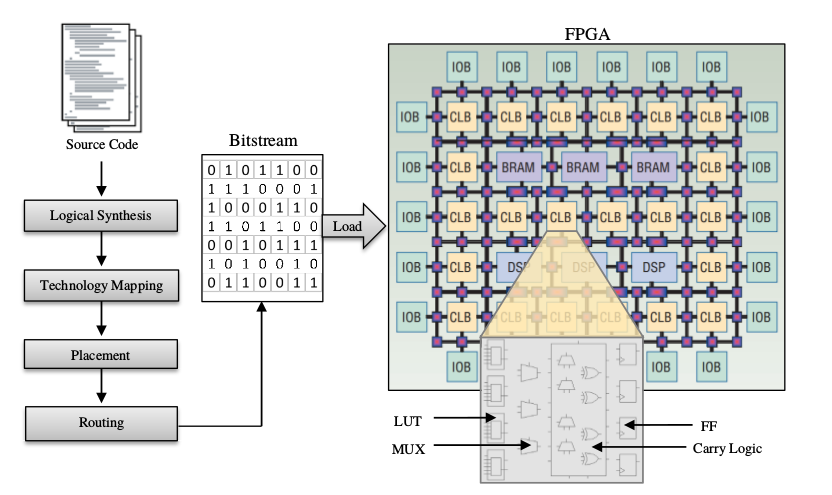
\includegraphics[scale=0.4]{figures/img/FPGA-structure.png}
   \caption{FPGA Structure and Design Flow~\citep{manuzzato2010single}}.
\label{fig:fpga-struct}
\end{figure}




The process starts with the design written
in a hardware description language (HDL), e.g., VHDL or Verilog. Next, the design is optimized and mapped into the FPGA’s available resources through logical synthesis,
technology mapping, placement, and routing. Finally, the generated bitstream downloaded into the device, and the device starts functioning according to the designer design.


Like any other semiconductor device, FPGAs are sensitive to radiation effects~\citep{hobeika2014multi}.
Mostly, these effects depend on the technology used to store the configuration data.
The foremost concern for SRAM-based FPGAs is
SEUs within the configuration memory, because the configuration memory controls all the operations, e.g., data and control~\citep{manuzzato2010single}.
Upset configuration bits may change the logic and routing of the implemented system, as
shown in Figure~\ref{fig:seu}, leading to functional failures in an unpredictable way. Anti-fuse and flash-based
FPGAs offer a relative immunity to SEEs, but these devices have a lower logic capacity, and anti-fuse is only time programmable, making SRAM-based FPGAs more
suitable for complex systems giving facility of more frequent reconfiguration and adaptation~\citep{quinn2015validation, violante2004simulation}. 

Errors produce in the FPGAs due to SEU can be classified into two different categories - errors affecting the logic blocks and errors affecting the routing~\citep{sterpone2006new}. For the logic block, the SEU can produce the following errors~\citep{sterpone2006new}.

\begin{itemize}
\item LUT error: SEU modified the bit of the LUT.

\item MUX errors: SEU changed the configuration of the MUX in a logic block.

\item Flip-Flop error: SEU modified the configuration of an FF.

Routing resources are about the 80 percent of FPGA resources; SEE can create different phenomena that modifies the programmable Interconnect Points (PIPs)~\ref{sterpone2006new}.

\end{itemize}



\begin{figure}
 \centering
  \captionsetup{justification=centering}    
   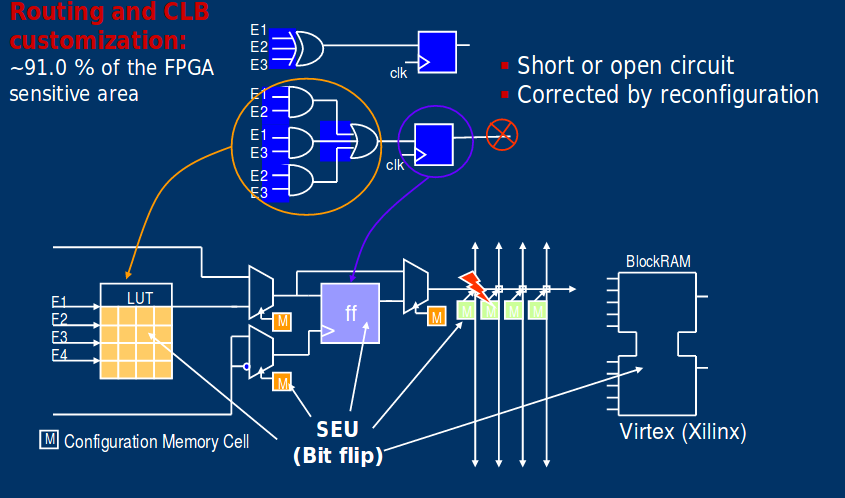
\includegraphics[scale=0.4]{figures/img/seu.png}
   \caption{Upset FPGA configuration bits may change the logic and routing~\citep{manuzzato2010single}}.
\label{fig:seu}
\end{figure}




%\subsection{Faults, and Failure}


\section{Design Verification by Fault Injection}




The second domain to understand in this project is designing, testing, and verification of the design (digital circuit) by fault injection on FPGAs. As we discussed before, SRAM-based FPGAs are particularly sensitive to SEUs. The configuration memory is the most sensitive part. By changing the configuration memory, may affect the overall functionality of the system. The work done so far to study the SEU effects on FPGAs, combines the emulation, simulation, and radiation testing.

\subsection{Emulation}

The purpose of fault emulation to reproduce as closely as possible radiation based results, evaluate the criticality of FPGA resources, analyze the impact of flipping the critical bits, find the faulty response of the circuit. Several works have been done so far deals with the analysis and emulation of SEUs in an FPGA which is done by flipping the bit in the configuration memory. 

The work presented in~\cite{hobeika2014multi} provide an emulation platform for the signature generation. This work is focused on the identification of the emulation zone,  fault list generation, SEU emulation, and result Analysis. The purpose of their work is to investigate the sensitivity of SRAM-based FPGAs for evaluating the effects of SEUs. In this paper, they also provide the results for the radiation based signature and simulation-based signature. They showed that simulation and emulation-based signatures could contain the same error values as obtained with radiation but their probability of occurrence could significantly different. The arithmetic signature for TRIUMF to emulation is 85.3\% for adder and 84.8\% for the multiplier. 

The work presented in~\citep{souari2015optimization, souari2016towards} deals about the fault injection into the FPGA configuration memory based on the sensitivity of the bits by considering that the "bits-at-one" are more sensitive to the "bits-at-zeros." They have developed a methodology to extract the list of "configuration bit addresses of the design LUTs" based on the essential bits file of the design named \textit{.ebc},  which can be extracted by the Xilinx \textit{BitGen} command.




An accelerated fault injection technique is presented in~\citep{di2014fault} based on the design essential bits provided by the \textit{bitgen}. Similarly, there are few other techniques availble for the fault emulation based on the random fault injection~\citep{faure2005single}.


The work proposed in the~\cite{hobeika2013flight} described a completed automated methodology to emulate SEUs on an FPGA efficiently. The authors used the reconfigurable flight control system as an application.
In this work, they are focused on the essential bits identification to speed-up the fault emulation and proposed on the new fault models.



The work presented in~\cite{quinn2015using} described the benchmark that can be used for the reliability and radiation effects study on FPGAs and microprocessors. 

%\begin{itemize}
%
%\item   {Classification of the configuration bits into subsets.
%        a.  Bits set to 1/0 of LUT.
%        b. Bits set to 1/0 configuring other than LUT.
%        c. Bits set to 1/0 configuring other resources not identified as  potentially critical by bitgen.}
%        
%        
%\item  {Estimating the number of critical bits of the set by randomly injecting faults in the bits of each set. This method helps to find the most critical zones of the FPGA.}
%
%\item {Prioritized the fault injection in the identified (step-2) most critical zones.
%These classification steps are done with the help of EBC and EBD files provided by the bitgen. The experimental results presented in [5] evaluated the SEU sensitiveness as well as bitgen efficiency. The results are evaluated between random fault injection with different prioritized bit subsets.  The first observation authors concluded - the bitgen did not accurately identify all the critical bits meaning the bitgen limitations. Second authors did the prioritizing the most sensitive subset. It would involve exhaustive fault injection. The authors used fault injection to get an estimated number of critical bits as well as the related estimation error. They used the term critical bit error estimate (CBEE). The authors claimed the CBEE observed for the random approach is higher than the observed under the bits subsets.  The ratio of observed critical bits (ROCB) observed for the random injection is far less than the different bits subsets.}



%\end{itemize}

\subsection{Simulation}

Simulation-based testing is low cost and flexible, but it is difficult to get the accurate results. For simulation-based testing, the work presented in the~\cite{violante2004simulation} described an approach for fault injection based on the simulation during early design phase when the hardware system is not ready.  This work helped to find the probability for an SEU to change the behavior of a given circuit.

The work presented in~\ref{robache2013methodology} demonstrates how faulty behavior --- signatures allow building high-level models, i.e., high-level faulty model, e.g., fault model in MATLAB simulink, that reflects the faulty behavior of a combinational circuit represented at gate-level. The fault injection tool is used named  LIFTING.  The purpose of this tool is to inject different types of faults on a circuit at gate-level. The tool used the stuck-at-0 and stuck-at-1 in each node of the design. The LIFTING is a simulation-based gate-level fault injection tool that used the circuit netlist file, e.g.  *.v file. The work presented in this paper helps to make a faulty block with Simulink that reads a signature and generates errors according to the distribution.

\subsection{Radiation Testing}
Radiation testing is an expensive approach and requires a state-of-the-art facility. The work presented in~\cite{hobeika2014multi} described the effects of radiations on a circuit at the circuit-level. In this work the also compared the results which are expressed as signatures based on fault simulation, emulation, and radiation testing of the FPGA. They want to capture and regenerate the faulty behavior occurs due to SEUs early in the design process. 

The work presented in~\citep{dsilva2015neutron} used the Flash-based FPGA under neutron beam to observed the SEE in avionics applications. They observed; the failure-in-time rate for flip-flops, SRAM cell, PLL are reasonably low. They proposed the SEL testing procedure and observed Flash-based FPGAs are immune to SEL. 

In~\citep{maillard2015neutron} authors tested the UltraScale Kintex FPGA under neutron and proton beam. They examined the single event upset response of the FPGA. They presented the result regarding a failure in time calculation. They observed that there are less than 0.1\% uncorrectable events. 


Software benchmark radiation testing is done on the flash-based micro-controller. They also tested a ferroelectric-memory-based micro-controller, two ARMs, and GPUs. These components are tested with both mitigated and unmitigated codes. The results reported in the paper for two different microcontroller and two ARMs cores. For microprocessors: they observed the FITs are very small. In some cases, there is no error from the code during many days of testing. 










%\subsection{Benchmark for Radiation Testing}
%The suitable selection of the benchmark for the radiation testing of microprocessor and FPGAs is a recently topic of ongoing research. The benchmarks are used to evaluate the performance under different architectures, technology, and compiler. There is no such standard benchmark employed to study microprocessor and FPGAs under the effects of radiations; make it difficult to assess the changes in fabrication technology, architecture, and circuitry. The work presented in~\cite{quinn2015using}described the software and hardware benchmark under the neutron test data. The unavailability of the such a benchmark for testing because radiation hardness assurance techniques are applied only to circuit layouts or manufacturing process. There is no standard test circuits available, researcher, used flip-flop or D-latches to compare their results. In recent years, radiation effects community shown interest to develop a standard set of circuits that include complex and realistic algorithms and can be adapted to different FPGAs.  Currently, without standard benchmark researcher used the following approach for testing:
%
%\begin{itemize}
%
%
%\item Homemade Design.
%\item Circuits from Opencore.
%\item Proprietary designs.
%\end{itemize}
%
%
%The problem with this approach as no two organizations used the same set of codes or circuits, difficult to make the comparison. There is a need for collaboration to make a suitable set of benchmark for reliability application and study the effects of radiation under the same conditions. The criteria used to set a standard benchmark including:
%
%Repeatability of benchmark tests.
%A representative of deployed computing workload.
%Availability of fixed input vectors.
%Cross-platform implementation.
%The ability to repeat test itself is an important part of the standardized testing. By repeating the algorithms, the input test vector, the compilation, the synthesis setting help researchers to have the enough information. It is necessary to provide a wide variety of realistic algorithms so that the system can be tested as likely to the realistic application. Defining the input test vector is an essential step because many hardware errors can be observed under the specific set of the test vector. It is an open question which input test vector should be adopted, under the specific set of criteria. Finally, the implementation of the algorithms in portable languages help to use the same set of codes on the different platform. For example, assembly language for the microprocessors limit the ability to compare and port codes on the different platform. But the hardware benchmark developed in VHDL can ease the problem; the same circuit can be ported to any FPGA.
%
%\textbf{FPGA Radiation Benchmark}
%
%The FPGA benchmark mentioned in this paper is ITC'99 which is well defined ATPG benchmark. This benchmark meets all the requirements, e.g., realistic algorithms, input vectors, scalability, and portability. The circuits are implemented in the HDL so that it can be ported to different FPGAs. The first 15 circuits from the ITC'99 are adopted for the benchmark as shown in Table I.

%\textbf{Software Radiation Benchmark}
%
%The software radiation benchmark is harder to design than the FPGA radiation benchmark. The development of the standard set of algorithm that can be ported on different architectures would be a challenging task e.g., porting an algorithm to 16-bit microcontroller to GPU. The authors are interested in the software benchmark where the computational load can be divided into the parallel processes or run on a single core. The commonly used software benchmark comprises of fast fourier transform, matrix multiplication and quick-sort algorithm as they are commonly used in many applications and useful for the evaluating the reliability of parallel processors. The software benchmark comprises the following code.
%
%\begin{itemize}
%\item AES-128;
%\item Cache test;
%\item FFT;
%\item Hotspot;
%\item HPCCG;
%\item Matrix Multiply;
%\item Quicksort
%\end{itemize}










%\section{Fault-detection, mitigation and correction in the FPGA }


%The impact of SEUs on SRAM FPGA devices has been studied in~\cite{bellato2004evaluating}. Many  techniques  have  been  proposed to provide highly reliable FPGA devices, e.g. radiation-hardened FPGAs~\cite{rockett2007radiation}, in-order to lower the effect of radiation-induced SEUs. However, radiation-hardened  SRAM  FPGAs  typically have  a  low  density, and  they  only  may  lower  the  probability of SEUs to occur but  not  completely avoid  them. Therefore, non radiation-hardened FPGAs, like the  Xilinx Kintex-7, are evaluated under a harsh radiation  environment~\cite{wirthlin2014soft}. Even on radiation-hardened FPGAs, the SEU rate in a low-earth orbit flight experiment can be up to 16 events per day~\cite{quinn2012orbit}. A wide  variety  of  SEU  fault  mitigation  techniques  for SRAM-based  FPGAs  have  been  proposed  during  the  past years. These techniques can be categorized into module redundancy techniques such as triple modular redundancy (TMR)~\cite{lyons1962use} and techniques that use scrubbing of the FPGA configuration memory~\cite{heiner2009fpga}. Also the combination of  both techniques has been shown to be able to increase the reliability of FPGA modules significantly ~\cite{ostler2009sram}. FPGA-based TMR approaches replicate a given module which shall be protected either statically or dynamically~\cite{angermeier2011runtime}. The different granularities of voted replicas  are evaluated in~\cite{bolchini2007tmr}. However, no upset rates and consequential no reliability figures are provided. Nevertheless, TMR techniques are  known to often cause an excessive and unacceptable overhead in terms of power  consumption and area. Since the intensity of a cosmic rays is not constant but may vary over several magnitudes depending on the solar activity, a worst-case radiation protection is far too expensive in most cases. A self-adaptive system is proposed in~\cite{glein2014self}, which monitors the current SEU rate and exploits the opportunity of partial reconfiguration of FPGAs to implement redundancy such as TMR on demand. 

%Memory scrubbing is a well-known correction technique for the configuration memory of SRAM-based FPGAs. It consists on re-writing the configuration memory after the FPGA is configured to restore its original content. It is often a transparent operation for the running application. This is possible because modern FPGAs offer a dynamic partial reconfiguration (DPR) feature. The circuit that enables the scrubbing is commonly named scrubber. Additionally, readback is the process of reading the configuration memory of the FPGA after it is configured. Both processes (readback and scrubbing) can be used to implement different scrubbing methodologies as shown in~\cite{herrera2013design}. Scrubbing can be implemented using an internal or external interface as shown in~\cite{berg2008effectiveness}. When external interface is used, the scrubbing logic is implemented outside the FPGA. In the case of Xilinx FPGAs several external interfaces are available; however, the Select MAP interface has the highest data throughput. On the other hand, there is only one internal interface named ICAP~\cite{xilinx}. This internal interface can be accessed from the reconfigurable logic of the FPGA and it is a replica of the Select MAP interface. Also scrubbers can be implemented in software or hardware. The scrubbing process can be implemented using a microprocessor with the advantage of a high flexibility to implement different complex scrubbing methodologies but with lower configuration speeds and lower energy efficiency.



\section{Fault Models}


The last domain of this work is related to the fault models, and fault analysis. We further divided into three different categories: behavior domain, transformation and circuit domain and provide a related work on each domain separately.


\subsection{Behavioral Domain:}




In~\citep{svenningsson2010model}, authors, presented the idea that how model-based fault injection can be utilized to
simulate the effect of hardware related faults in embedded systems. Model-level and hardware-level
fault behavior comparison is presented. They performed the emulation on the micro-controller. They developed a tool which changed the bit value in the register or memory cell through assembly language program. They modified the code through assembly tools and analyzed the behavior of the fault.

In~\citep{hayne1999behavioral}, authors, proposed two tools, which facilitate the fault simulation of behavioral
models, described using VHDL. The tool is the Behavioral Fault Mapper (BFM). The BFM algorithm
accepts a fault-free VHDL model of the design (combinational circuit) and a fault list of N faults from
which it produces N faulty models. The assumed eight different fault models, e.g., Stuck-Then, Stuck-Else,
Assignment Control, Dead Process, Dead Clause, Micro-operation, Local Stuck-data, and Global Stuck-data. 

In~\citep{chen2017fault} authors, proposed the fault propagation process between the different subsystem of the
main system, combined with the finite state machines. This work is based on the FSM and fault propagation model. In this work, authors analyzed how the fault comes in one sub-system effects the others and leads towards the overall failure of the system. They calculated the Mean Time Between Failure (MTBF).


The work presented in ~\citep{mirzadeh2014modeling} proposed a fault behavior model developed with a neural network
concept. The neural network is used to synthesize the faulty output of a
circuit at a high-level of abstraction. They used a neural network to replicate the faulty behavior of the circuit in the presence of the fault. The idea is good to make a model with neural networks. But the work is done based on simulations only, no hardware experimental results reported. Moreover, the author claimed in their "proposed methodology chapter"  --- "The goal of developing a behavioral fault model of a circuit is to create a library of faulty components reusable at high-level of abstraction." But they didn't provide any results for the library of faulty components.


In~\citep{janschek2017errorsim} authors proposed the high-level fault behavior model. This work used for the error propagation analysis. They developed a tool that has the ability to simulate different fault-models, e.g., offset, stuck-at-fault, noise, delay, package drop, and bit-flip. They used the passenger jet Simulink model for the experimental purpose. They analyzed the critical and non-critical sensor fault for the closed-loop passenger jet control sequence.

In~\citep{hobeika2013flight} authors presented the new fault model that can be used by the designer at an earlier stage in the design process. In this work, they used the adaptive control model and did the SEU emulation on it. They found the new fault model, e.g., control amplification, sign inversion, etc. They also provide the information about the design essential bits and the bits used for the fault emulation.

The work presented in~\citep{thibeault2013library} based on the C/C++ description of an application. They used the technique to convert the circuit into control and data flow graph (CDFG) file, then used the resource estimation tool, to find the resources required to implement an application on an FPGA. This work is based on the .xdl and .ncd file of the design provided by the Xilinx tools, which are no more compatible with new FPGAs.


The work presented at the behavioral level did not have the insight information of the how fault influences the hardware at the circuit level. For example, the work presented in~\citep{janschek2017errorsim} supposed the fault distribution is normal, exponential, Poisson, Weibull. The most of the research work has been done is related to the transient fault analysis, soft error rate (SER) analysis and error prediction, error propagation,and failure-in-time calculations.


The methodology we present in this thesis based on the fault emulation at the circuit-level and abstract it to the high-level. Details are in the Chapter~\ref{approach}, in which detail information given about the model abstraction at the high-level based on the low-level circuit behavior.


\subsection{Transformation Domain}



There has been a lot of work done for the analysis of the faulty circuits and error propagation based on the techniques that involve the transformation of the circuit or design into some other equivalent domain, e.g., Binary Decision Diagram, then analyze the fault and error behavior. Compute the SER  and error probabilities.

The work presented in~\citep{ubar2014modeling} is based on the simulation of the faulty circuit, authors transformed the circuit into their required tool format, i.e., structurally synthesized BDD, then they
insert the fault on different nodes to calculate the SER. 


Modeling the probabilistic behavior of the Finite State Machine, calculating the steady state
behavior of the circuit and used for estimating the switching activity of the circuit for
power evaluation presented in~\citep{hachtel1996markovian}. They showed how steady-state probabilities of very large FSM’s could be computed by
symbolic ADD-based algorithms. In this work, authors need to convert the FSM into respective BDD model to perform the fault simulation.


In~\citep{shazli2011high}, soft error rate  computation problem is modeled as a Boolean
Satisfiability (SAT) problem and SAT solvers are used to compute SER for combinational and
sequential circuits. They used an automated flow to convert combinational and sequential behavioral
descriptions into equivalent SAT instances and analyzed them for SER.



In~\citep{miskov2007mars}, the symbolic framework based on Binary Decision Diagram / Algebraic Decision
Diagram is presented for sequential circuit analysis. They determined output gate susceptibility to error. The error is calculated at the transistor level. They also estimate the gate error probabilities.


The limitation of working in this domain require converting the circuit into a tool with many assumptions. The most of the work is based on the mathematical and analytical expressions. This requires deriving the mathematical expressions for the fault model in the tool converted format. This work also needs to assume the fault will create an erroneous output, plus its too hard for complex circuits to transform and derive their mathematical expressions.


\subsection{Circuit Level}


In~\citep{li2016monte} authors presented a  Monte Carlo technique for the soft error analysis of the sequential
circuits. They performed the logic simulation for latch-level error propagation to estimate the SEUs. This work is mainly focused on the SEUs convergence meaning after how many clock cycles the circuit becomes fault free.
They insert the fault into the simulator and observe it to the output. Apply the Monte Carol technique
to find the number of samples and the time for the estimation of the error.
  
  

The key idea behind~\citep{ebrahimi2015comprehensive} is to present the result for SER analysis on an embedded
processor. Their platform employs a combination of models at a device level, a gate level, and architectural level. They used the
processor core and derived all the results via simulation under the assumption of the fault. While using processor core under the radiations, the primary concerns is for the cache memory instead
of the core itself.


The technique used in~\citep{ranjan2014aslan} is to estimate the output quality of a faulty circuit. They used the concept
of unrolling the circuit with each clock cycle and compares faulty unrolled circuit with the original circuit and find the errors.
The cost of unrolling and analyzing error metric also increase
with circuit complexity.

In~\citep{yu2010scalable}, authors developed novel and efficient ways to examine a behavior of a circuit. They model the impact of soft errors and estimate the circuit reliability. Their method is based on the probabilistic transfer matrices to calculate signal and error probability distributions in the
sequential circuits at the logic level. This work is mainly focused on finding the signal probabilities at the gate level. They partitioned the combinational part of the sequential circuit, and then find the probabilities of each gate.


In~\citep{miskov2007mars},  authors estimated the likelihood that a SET in a sequential circuit will lead to errors
in clock cycles following the particle hit, and found after the hit (which is an assumed fault) how many clock
cycles needs to get the SER below the threshold level which they set. The main idea is to do symbolic modeling and efficient estimation of the susceptibility of a sequential circuit to soft errors.




In~\citep{lingasubramanian2010probabilistic}, authors calculated the maximum error in digital circuits and found the respective
worst-case input pattern, through a posteriori hypothesis, using a Shenoy-Shafer algorithm.
They showed the importance of handling maximum error behavior for achieving fault tolerant
computing machines. .

In~\citep{miskov2008modeling}, Markov chain for the steady-state behavior of the sequential circuits, a Symbolic framework
based on the BDD/ADD is presented. They did the Single Error Rate evaluation, purposed to do
for the gate sizing, find the gate size that has the highest soft error impact based on this recommend
different gate size for the transistor technology. 
 




In~\citep{das2007monitoring}, error monitoring scheme to detect the transient error is presented. The idea presented in this work has worth to compute the error for each stage
independently. But they didn't provide they experimental setup details, to analyze the benefits and overhead of this technique.

In~\citep{asadi2005soft}, they provided the multi-cycle analytical framework to analyzed the multi-cycle error
propagation. The major limitation of their work is the measuring unit they used  “mean time
to manifest error.” The standard terminology for this kind of work is SER. This is the simulation work,
with the assumption that the fault will occur in the flip-flop and proceed to another flip-flop. They did not
consider the fault occurred in the combinational logic of the sequential circuit.

In~\citep{miskov2010multiple}, authors presented an idea to analysis the susceptibility of the circuits. The analyzed the outputs
errors originating from the single or multiple fault transients. They are keener to find the part of
the circuit that has the highest error generating probability.







The work is done in this domain used simulation setup for error calculation, assumed fault occurred, supposed the glitch size, and assigned the
probabilities for fault propagation in the HSPICE simulator. Authors make the model of the faulty circuits, analyzed them using modeling techniques, compare results with the simulations results derived by using the
HSPICE. 

They also assumed that an error occurs only in the first clock cycle of a w-cycle simulation with
no new errors occurring in subsequent cycles which also underestimates the usability of this work.  There is one more bottleneck if the circuit size and the number of primary
inputs and outputs grow linearly with the number of simulated cycles, and memory usage becomes
unmanageable after a few simulated cycles.










\label{related}





%%% Local Variables:
%%% mode: latex
%%% TeX-master: "../Document"
%%% End:
